\documentclass[12pt]{report}

\usepackage[italian]{babel}
\usepackage[latin1]{inputenc}
\usepackage{url}
\usepackage{biblatex}
\usepackage{amsmath}
\usepackage{graphicx}
\usepackage{caption}

\hyphenation{ransac}
	
\bibliography{bib}

\begin{titlepage}
\begin{center}

\HRule \\[1.1cm]

\textsc{\Large Progetto di \\ Image Analysis and Synthesis \\ e \\ Argomenti avanzati di analisi di immagini}\\[0.5cm]
\textsc{\large A.A. 2010/2011}\\[0.5cm]

% Title
\HRule \\[1.5cm]
{ \huge \bfseries iaasFog}\\[0.4cm]
{ \huge \bfseries Analisi della visibilit\'a in condizioni di nebbia}\\[0.4cm]
\HRule \\[1.5cm]

% Author and supervisor
\begin{minipage}{0.4\textwidth}
\begin{flushleft} \large
Stefano \textsc{Cadario}, \\ mat. 724842\\
Luca \textsc{Cavazzana}, \\ mat. 734498
\end{flushleft}
\end{minipage}
\begin{minipage}{0.4\textwidth}
\begin{flushright} \large
Prof.~Vincenzo \textsc{Caglioti}
\end{flushright}
\end{minipage}

%\vfill
\HRule \\[3cm]

% Bottom of the page
{\large 10 maggio 2011}

\end{center}
\end{titlepage}

\begin{document}
%\maketitle

\tableofcontents

\chapter{Introduzione}

L'obbiettivo del progetto \`e estrarre un parametro numerico indicante la visibilit\`a in caso di nebbia utilizzando esclusivamente delle immagini riprese da una telecamera montata su un'automobile. La tecnica utilizzata si basa sull'analisi della variazione del contrasto delle features individuate in ogni frame dell'immagine con il fine di trovare il parametro $\lambda$ della funzione

$$k_fe^{-t/\lambda}$$

\noindent Tale funzione deriva da una prima analisi teorica del problema in questione: il parametro $k_f$ rappresenta il massimo livello di contasto di una generica feature $f$ in condizioni di visibilit\'a ideali, mentre $\lambda$, globale, rappresenta il tempo medio d'impatto per una feature che sta emergendo dalla nebbia, prendendo come riferimento il valore di contrasto come pari a $k_f/e$.\\

\noindent I problemi affrontati nel corso di questo progetto consistono nello sviluppo di una tecnica performante per l'individuazione e il tracking di features il cui movimento relativo sia consistente con quello del veicolo, e trovare un metodo per il calcolo del contrasto e la stima dei parametri in questione sufficientemente robusto ai livelli di rumore sui dati.\\
	 	
\noindent Un simile sistema potrebbe essere integrato fra i sensori di un veicolo, monitorando l'idoneit\`a della velocit\`a di crociera rispetto alle condizioni di visibilit\`a e ai tempi di reazione del conducente. Nel campo emergente dei veicoli autonomi, similmente, potrebbe vincolare il valore massimo di velocit\`a in base ai tempi di risposta, oppure potenziare la consapevolezza del sistema di analisi d'immagine fornendo un parametro per la stima della qualit\`a dei dati a seconda della distanza dell'elemento da cui sono state ricavati.



\chapter{Implementazione}

\section{Tracking delle features}


\noindent Il tracking delle features\footnote{All'interno di questo documento con il termine ``feature'' ci si riferisce ad una sequenza di corner associati ad uno stesso dettaglio nella scena in frame successivi.} deve individuare il maggior numero di features in ogni immagine, e nel contempo escludere gli outliers che influirebbero nei passaggi successivi dell'elaborazione.\\
L'elaborazione dei frame avviene in modo inverso rispetto al tempo, in modo da individuare le features quando sono ben visibili per poi inseguirle nei frame temporalmente precedenti, dove il riconoscimento \`e pi\`u difficoltoso a causa della nebbia.\\

\noindent Ad ogni frame viene eseguita la funzione \verb|cvGoodFeaturesToTrack| che individua la posizione dei corner con autovalori pi\`u alti e quindi con maggior probabilit\`a di essere individuati nei frame successivi. Nel frame successivo vengono quindi inseguiti utilizzando la funzione \verb|cvCalcOpticalFlowPyrLK|, che utilizzando l'algoritmo iterativo di \emph{Lucas-Kanade} ricalcola la nuova posizione di ogni feature.\\

\noindent Prima di aggiungere alla sequenza il nuovo punto individuato vengono effettuati dei controlli di coerenza: la nuova posizione deve avere direzione concorde con i punti antecedenti ed il nuovo passo deve essere maggiore dei precedenti. Una sequenza di corner \`e considerata valida se \`e inseguita per almeno cinque frame (per ottenere una migliore approsimazione del birapporto), in caso contrario viene eliminata. Se la feature \`e valida viene eseguito un controllo sulla cross-ratio dei punti, che deve essere prossima a 4/3. I punti trovati saranno comunque soggetti ad errori di posizione dovuti a diversi fattori e quindi non collineari: per rimediare viene quindi calcolata la retta di regressione, su cui verranno proiettati i punti per l'analisi del birapporto.\\

\noindent Il tracking dei corner diventa sempre pi\`u difficoltoso all'avvicinarsi al vanishing point a causa del calo dei livelli di contrasto dovuti alla nebbia, che riduce la possibilit\`a di individuazione; per ovviare a questo problema vengono calcolate le posizioni teoriche delle features utilizzando i punti nei frame precedenti e la cross ratio nota. Il tracking di una feature ha termine quando non si hanno pi\`u frame disponibili oppure quando lo step del nuovo punto \`e inferiore a $0.5$ pixel.

\section{Calcolo del vanishing point}
La posizione del vanishing point riveste un ruolo fondamentale nella risoluzione del problema poich\'e viene coinvolto sia nel filtro degli outliers, sia nel calcolo del tempo d'impatto di ogni feature.\\

\noindent Inizialmente \`e stato implementato un algoritmo che prevedeva l'individuazione di tutti i punti di intersezione tra rette e da questi ricavare il punto che minimizza la distanza con tutti gli altri. Questo approccio, sebbene abbia dato buoni risultati, si \`e rivelato troppo lento a causa della complessit\`a eccessiva del problema che richiedeva fino a $15$ secondi di elaborazione per $200$ features (complessit\`a $O\left(n^4\right)$).\\

\noindent Dopo un primo tentativo di ottimizzare l'algoritmo gi\'a esistente si \`e deciso di tentare un approccio completamente nuovo sfruttando RANSAC:

\begin{itemize}
\item	Ad ogni iterazione viene eletto casualmente un possibile candidato vanishing point calcolando l'intersezione delle rette rappresentanti due features, con il solo vincolo di essere all'interno del field of view dell'immagine.
\item	Per ogni retta viene calcolata la distanza dal vanishing point candidato. Tali distanze vengono ordinate in un vettore, la cui mediana sar\`a il rank associata a quel particolare vanishing point.
\item	Se il nuovo vanishing point ha un rank migliore dei precedenti viene eletto come nuovo best vanishing point.
\item	Il ciclo termina quando vengono analizzati un numero di intersezioni ritenuto sufficiente (il $5\%$ di tutte le possibili intersezioni tra rette).
\end{itemize}

\noindent Vengono infine scartate le features la cui retta di regressione dista pi\`u della distanza mediana rispetto al vanishing point eletto, in quanto probabili outliers (viene mantenuta quindi solo la met\'a delle features).

\begin{figure}
	\begin{minipage}[b]{0.5\linewidth}
		\centering
		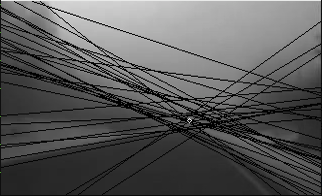
\includegraphics[scale=0.6]{images/iaasBefore.png}
		\captionof{figure}{Vanishing point calcolato mediante RANSAC.}
		\label{fig:vpBef}
	\end{minipage}
	\hspace{0.5cm}
	\begin{minipage}[b]{0.5\linewidth}
		\centering
		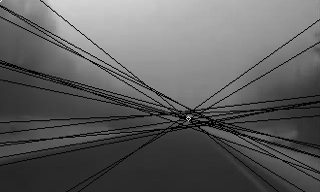
\includegraphics[scale=0.6]{images/iaasAfter.png}
		\captionof{figure}{Linee di fuga coerenti con il vanishing point calcolato.}
		\label{fig:vpAft}
	\end{minipage}
\end{figure}

\noindent L'algoritmo applicato a diversi set di dati ha restituito buoni risultati con tempi notevolmente ridotti (circa $1$ secondo di elaborazione per $200$ features) rispetto alla precedente implementazione meno efficiente (complessit\`a $O\left(n^2\log{n}\right)$).\\

\noindent Opzionalmente la posizione del vanishing point reale pu\`o essere affinata utilizzando SVD con il $50\%$ delle rette pi\`u vicine al vanishing point trovato in precedenza.\\

\begin{center}
	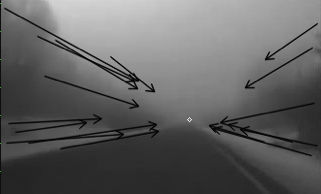
\includegraphics[scale=0.50]{images/iaasAfterArrow.png}
	\captionof{figure}{Flusso delle features inseguite.}
	\label{fig:vpAftArr}
\end{center}

\section{Calcolo del tempo all'impatto}

\noindent Dato un set di punti di coordinate $A$ e $B$ rappresentanti una feature in differenti immagini e conoscendo il frame rate $f$ delle telecamera \`e possibile calcolare il tempo d'impatto, ossia l'istante in cui la feature attraverser\`a il piano immagine, mediante il birapporto

$$ cross(i,a,b,v) = \frac{\overline{ia}}{\overline{ab}}\frac{\overline{av}}{\overline{iv}} = \frac{\overline{i'a'}}{\overline{a'b'}}\frac{\overline{a'v'}}{\overline{i'v'}} $$

\noindent Essendo nel mondo reale le distanze rispetto al vanishing point infinite, cos\`i come quelle rispetto al piano della telecamera nelle immagini, la formula si semplifica in

$$ \frac{\overline{ia}}{\overline{ab}} = \frac{\overline{a'v'}}{\overline{a'b'}} $$

\noindent Dal momento che $\overline{a'v'}$ e $\overline{a'b'}$ sono noti, ed essendo $ab$ la distanza percorsa dal veicolo fra le due immagini ($velocit\`a/frame rate$), il tempo d'impatto pu\`o essere ottenuto come

$$ t_{i} = \frac{\overline{a'v'}}{\overline{a'b'}}\frac{\overline{ab}}{v} = \frac{\overline{a'v'}}{\overline{a'b'}}*f^{-1} $$

\section{Calcolo del contrasto}

\noindent Per il calcolo del contrasto nell'intorno delle features sono stati presi in considerazione diversi approcci: oltre alla formule di Michelson e Weber, gi\`a sfruttate nelle precedenti fasi del progetto, \`e stato deciso di introdurre anche Root Mean Square, che calcola il livello di contrasto secondo la formula

$$ c\left(I_{M\times N}\right) = \sqrt{\frac{1}{MN}\sum_{i=1}^N\sum_{j=1}^M(i_{ij}-\bar{I})^2} $$

\noindent Dal momento che nel calcolo del valore contribuiscono tutti i pixel all'interno della finestra tale formula risulta essere molto pi\`u resistente al rumore rispetto alle precendenti, il cui risultato risulta essere dipendente dall'errore sul singolo pixel centrale per Weber, e dall'errore sui valori di min e max per Michelson.\\
\noindent Confrontando i valori ottenuti calcolando i livelli di contrasto utilizzando i diversi metodi si nota come RMS tenda a generare curve pi\`u smooth.

\begin{center}
	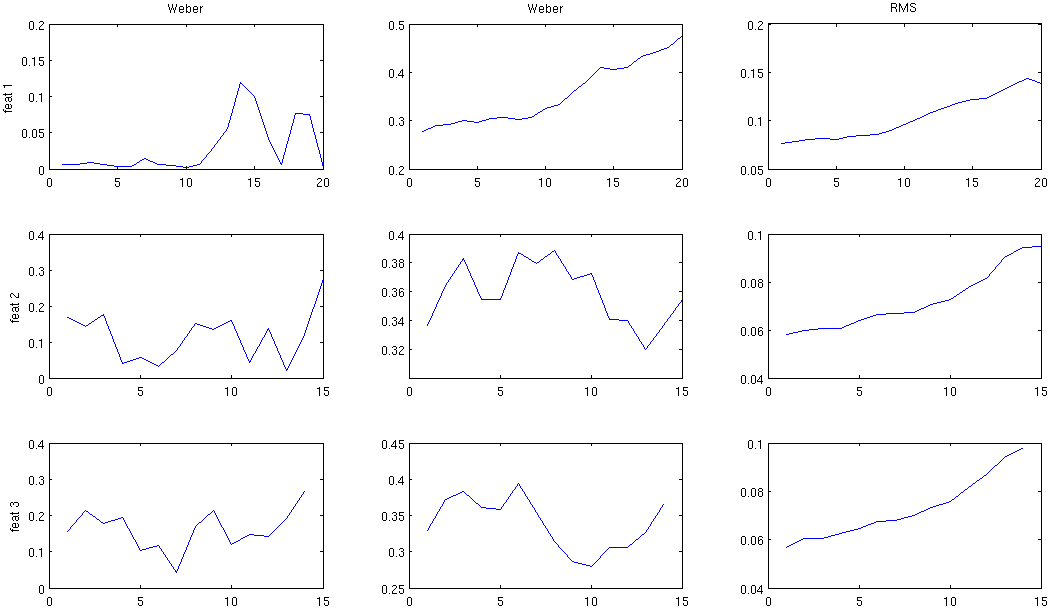
\includegraphics[scale=0.60, angle=90.0]{images/compContr1.png}
	\captionof{figure}{confronto fra i valori di contrasto ottenuti mediante i differenti approcci.}
	\label{fig:contr01}
\end{center}
\begin{center}
	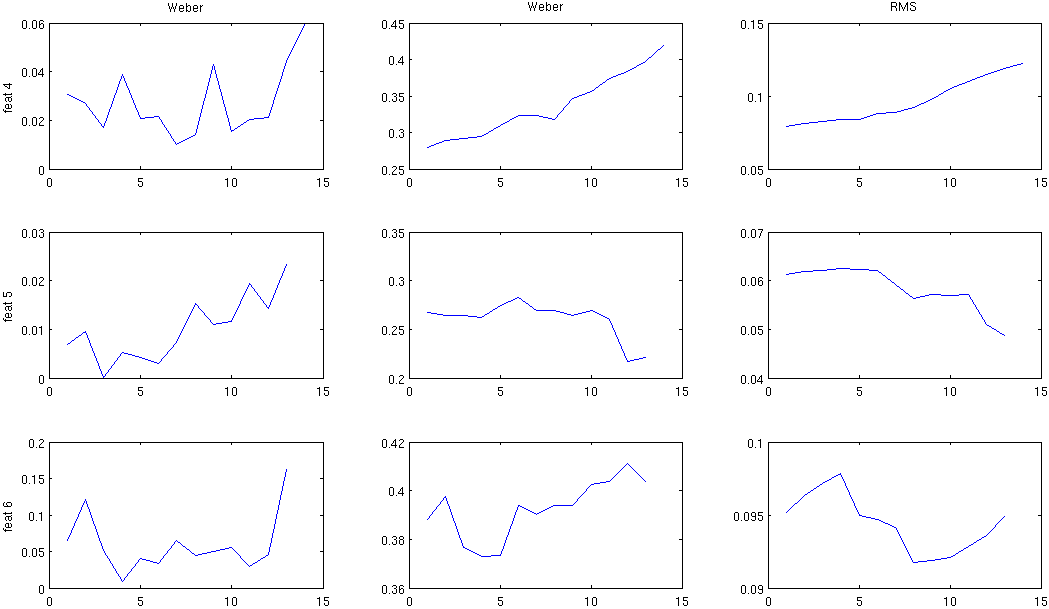
\includegraphics[scale=0.60, angle=90.0]{images/compContr2.png}
	\captionof{figure}{confronto su nuove features.}
	\label{fig:contr02}
\end{center}
\begin{center}
	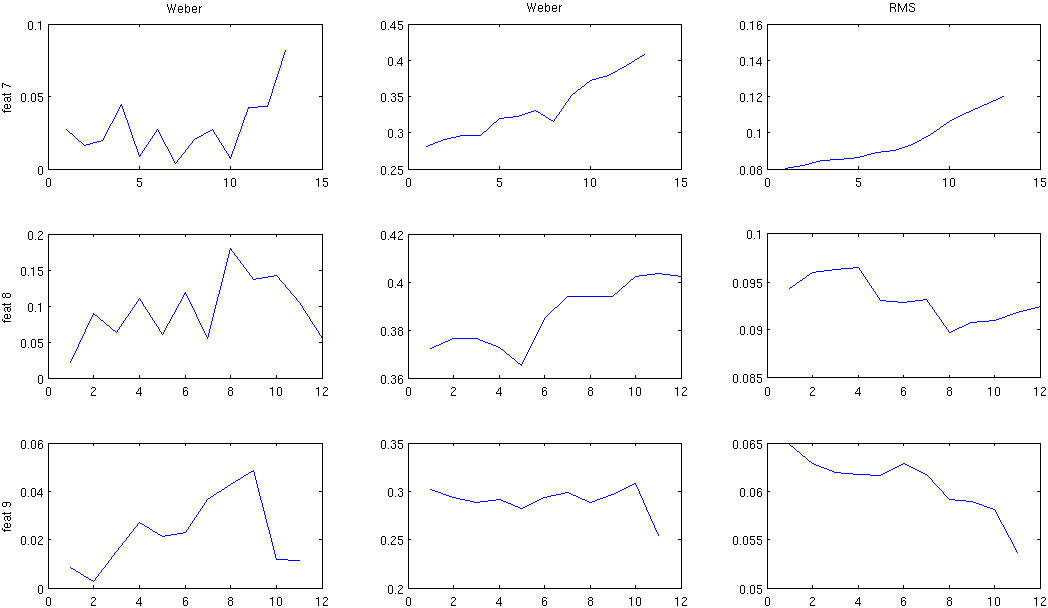
\includegraphics[scale=0.60, angle=90.0]{images/compContr3.png}
	\captionof{figure}{confronto su nuove features.}
	\label{fig:contr03}
\end{center}

\noindent Una particolarit\`a di RMS \`e che, al contrario delle altre tecniche, il risultato dipende dallo spazio di colori utilizzato per rappresentare l'immagine (facilmente risolvibile riscalando rispetto alla profondit\`a del colore).

\section{Stima dei parametri}

\subsection{Fitting di $\lambda$}

\noindent Una prima tecnica adottata \`e stata quella di sfruttare la funzione \verb|fit| di Matlab per estrarre il parametri $k_f$ e $\lambda_f$ che meglio descrivono ogni singola feature. Per ogni dato viene cos\`i calcolato l'errore rispetto alla curva generata, valore in base al quale verr\'a selezionata la met\'a dei dati migliori che verranno riutilizzati per approssimare nuovamente i parametri di una seconda curva esponenziale.\\

\begin{center}
	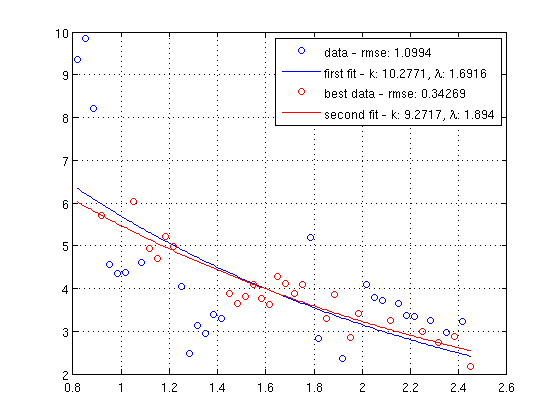
\includegraphics[scale=0.75]{images/twoFits.png}
	\captionof{figure}{Differenza fra due fitting consecutivi.}
	\label{fig:twoFits}
\end{center}

\noindent Fra i nuovi $\lambda_f$ calcolati vengono selezionati quelli associati al quartile delle migliori curve, scelte in base ad un valore, calcolato mediante diversi approcci:

\begin{itemize}
	\item	\emph{errore primo/secondo fitting}: l'errore viene calcolato come media dei rapporti fra l'errore e la proiezione del dato sulla prima/seconda curva approssimante calcolata.
	\item	\emph{variazione dell'errore}: nell'ipotesi di un buon set di dati la variazione dell'errore medio non dovrebbe essere molto grande. Viene quindi tenuta in considerazione la differenza fra gli errori calcolati (prossima a $0$ per buone features) o il rapporto (prossimo a $1$).
	\item	\emph{errore integrale}: sempre nell'ipotesi che per un buon set di dati la variazione fra le due curve \`e minima, viene calcolata la variazione sui parametri. Per aggregare i due valori viene considerata la differenza fra l'area delle due curve, calcolata come $$\left|\int^{\infty}_0\left(k_1e^{-t/\lambda_1} - k_2e^{-t/\lambda_2}\right)dt\right| =$$ $$= \left|\left[ k_2\lambda_2e^{-t/\lambda_2} - k_1\lambda_1e^{-t/\lambda_1} \right]^\infty_0\right| =$$ $$ = \left|k_2\lambda_2 - k_1\lambda_1\right|$$
\end{itemize}

\noindent L'ultimo approccio appare essere quello pi\`u robusto, ed \`e quello effettivamente selezionato nel programma. Il $\lambda$ globale viene cos\`i calcolato come la mediana di quelli selezionati.

\subsection{Normalizzazione mediante fitting di $k$ e RANSAC}

\noindent Un'altra tecnica sperimentata consiste nel calcolare il parametro $k_f$ della curva che minimizza l'errore su ogni singola feature.\\

\begin{center}
	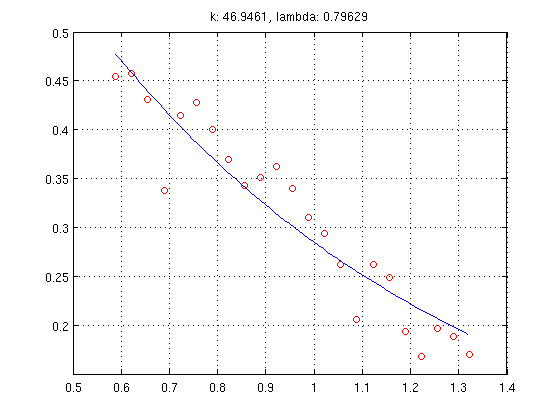
\includegraphics[scale=0.75]{images/fitting.png}
	\captionof{figure}{Fitting di una singola feature.}
	\label{fig:fitting}
\end{center}

\noindent Tale parametro viene utilizzato per normalizzare features con differenti valore di contrasto ``intrinseco'' (ovvero il massimo livello che otterremmo in condizioni ideali, senza nebbia): utilizzando $c_{i,f}/k_f$ possiamo cos\`i considerare sulla funzione discreta solo il contributo della nebbia, permettendoci di aggregare i dati di diverse features e stimare il parametro $\lambda$ globale sulla formula $$ c(t) = e^{-t/\lambda} $$ mediante RANSAC.\\
Questa implementazione di RANSAC seleziona a caso il $25\%$ dei set disponibili: i valori di contrasto vengono aggregati, ordinati in base al tempo d'impatto ed infine usati per stimare il $\lambda$ globale usando il parametro della curva approssimante. Per tale parametro verr\`a poi calcolato il set di consenso ed il relativo errore, iterando il processo come da manuale.\\

\begin{center}
	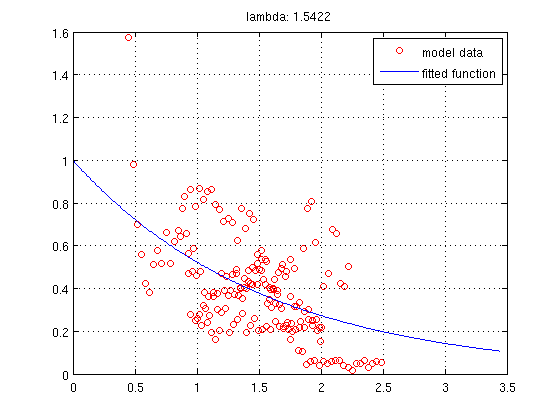
\includegraphics[scale=0.75]{images/tryLam.png}
	\captionof{figure}{Lambda candidato.}
	\label{fig:tryLam}
\end{center}

\noindent Il difetto di questo approccio \`e che vengono presi in considerazione anche dati molto rumorosi, che influiscono in parte sulla bont\`a del risultato.

\begin{center}
	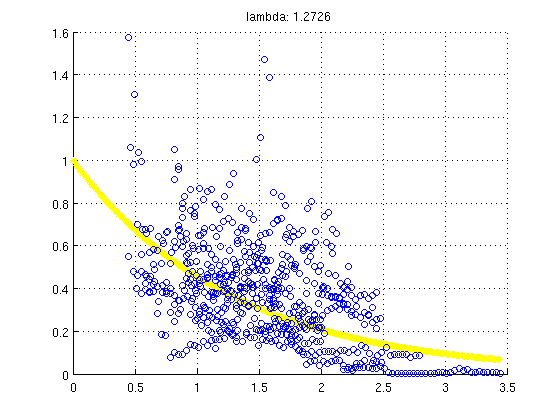
\includegraphics[scale=0.75]{images/ransacced.png}
	\captionof{figure}{Curva calcolata mediante RANSAC. In blu i contrasti ordinati sul tempo d'impatto.}
	\label{fig:ransac}
\end{center}




\subsection{Stima di $\lambda$ mediante minMax (deprecato)}

\noindent Definita la formula del contrasto per ogni feature come

$$ c_{i,f} = k_se^{-t_{i,f}/\lambda} $$

\noindent il parametro $k_f$ risulta essere costante all'interno di ogni singola sequenza di corner, mentre $\lambda$ \`e globale.\\
\noindent Sfruttando $k_s$ \`e possibile imporre la seguente uguaglianza fra due campioni di una stessa feature

$$ c_1e^{t_1/\lambda} = c_2e^{t_2/\lambda} $$
$$ \lambda = \frac{t_2-t_1}{\log\frac{c_1}{c_2}} $$

\noindent in modo da stimare il parametro $\lambda$ utilizzando i livelli di contrasto massimo e minimo (ed i relativi tempi all'impatto).\\

\noindent A questo punto viene introdotto un primo semplice criterio atto ad eliminare features eccessivamente rumorose: ricordando che i dati sono ordinati sul tempo d'impatto (e quindi il contrasto risulter\`a essere una funzione decrescente) vengono ignorate features la cui differenza fra gli indici dei valori di contrasto minimo e massimo non \`e sufficientemente grande (nel nostro caso dovr\`a essere superiore alla met\`a del numero di corners all'interno del set).\\

\noindent Successivamente si pu\`o procedere al calcolo di un $\lambda$ globale in base a quelli stimati calcolandone la media o la mediana.\\

\noindent Tale approccio tuttavia, per quanto computazionalmente leggero, \`e stato abbandonato a causa dell'eccessiva sensibilit\`a all'errore sui dati (dal momento che di sovente vengono selezionati come valori di min e max proprio degli outlier). Gli altri due approcci invece facendo uso di una maggiore quantit\`a di dati risultano essere pi\`u robusti, ma pagano in termini di prestazioni a causa della complessit\`a della fase di fitting delle curve.




\chapter{Risultati sperimentali}

\section{Calcolo del vanishing point}

\noindent Le figure \ref{fig:vp15}, \ref{fig:vp25} e \ref{fig:vp50} rappresentano il risultato dell'elaborazione dell'algoritmo sul calcolo del vanishing point su differenti set di immagini: l'algoritmo restituisce risultati tanto migliori quanto pi\`u sono le features disponibili, a loro volta dipendenti dal numero di frames; mentre per pochi frames (15) il calcolo del vanishing point \`e affetto da errori pi\`u o meno grandi, per tracking pi\`u lunghi ($>30$ frames) l'affidabilit\`a dell'algoritmo migliora notevolmente.\\

\noindent Nelle immagini poste a destra \`e possibile anche verificare come la met\`a delle linee di fuga individuate venga eliminata dal set, perch\'e troppo lontana dal vanishing point trovato.\\

\newcommand{\imTrackScale}{0.6}

\begin{figure}
\begin{minipage}[c]{0.5\linewidth}
	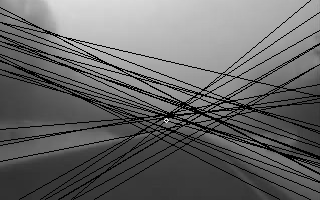
\includegraphics[scale=\imTrackScale]{images/bF_0000_15.png}
	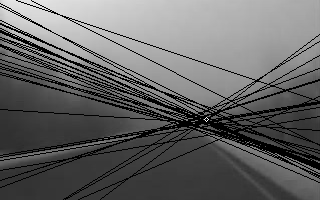
\includegraphics[scale=\imTrackScale]{images/bF_0020_15.png}
	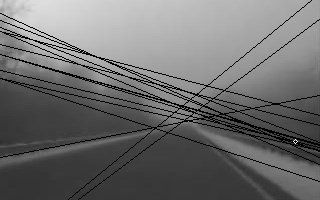
\includegraphics[scale=\imTrackScale]{images/bF_0040_15.png}
	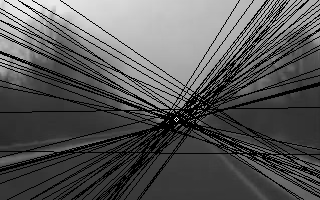
\includegraphics[scale=\imTrackScale]{images/bF_0060_15.png}
\end{minipage}
\begin{minipage}[c]{0.5\linewidth}
	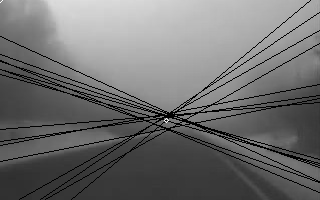
\includegraphics[scale=\imTrackScale]{images/aF_0000_15.png}
	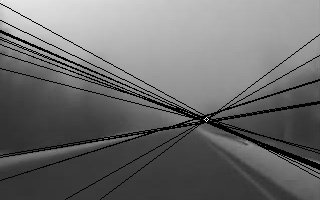
\includegraphics[scale=\imTrackScale]{images/aF_0020_15.png}
	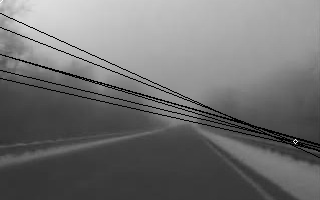
\includegraphics[scale=\imTrackScale]{images/aF_0040_15.png}
	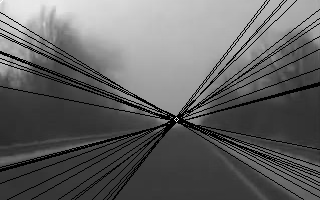
\includegraphics[scale=\imTrackScale]{images/aF_0060_15.png}
\end{minipage}
\caption[short]{A sinistra: linee di fuga per 15 frames a partire dalle immagini 0, 20, 40 e 60. A destra: stesse features dopo il filtro sul vanishing point.}
\label{fig:vp15}
\end{figure}

\begin{figure}
\begin{minipage}[c]{0.5\linewidth}
	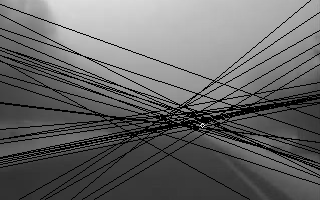
\includegraphics[scale=\imTrackScale]{images/bF_0000_25.png}
	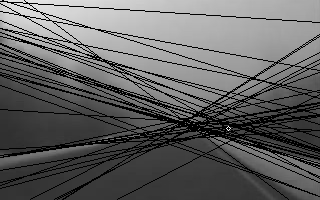
\includegraphics[scale=\imTrackScale]{images/bF_0020_25.png}
	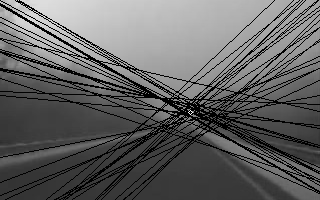
\includegraphics[scale=\imTrackScale]{images/bF_0040_25.png}
	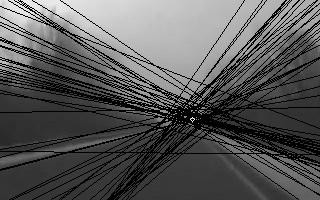
\includegraphics[scale=\imTrackScale]{images/bF_0060_25.png}
\end{minipage}
\begin{minipage}[c]{0.5\linewidth}
	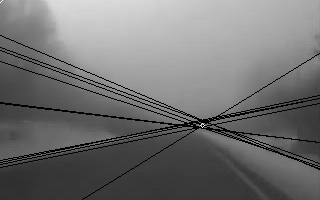
\includegraphics[scale=\imTrackScale]{images/aF_0000_25.png}
	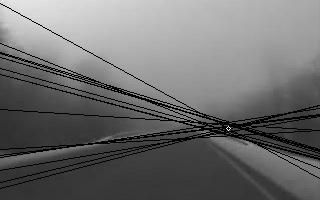
\includegraphics[scale=\imTrackScale]{images/aF_0020_25.png}
	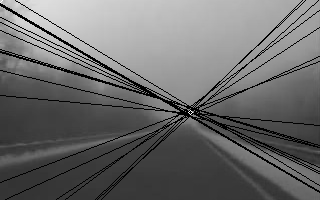
\includegraphics[scale=\imTrackScale]{images/aF_0040_25.png}
	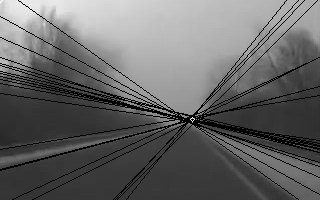
\includegraphics[scale=\imTrackScale]{images/aF_0060_25.png}
\end{minipage}
\caption[short]{A sinistra: linee di fuga per 25 frames a partire dalle immagini 0, 20, 40 e 60. A destra: stesse features dopo il filtro sul vanishing point.}
\label{fig:vp25}
\end{figure}

\begin{figure}
\begin{minipage}[c]{0.5\linewidth}
	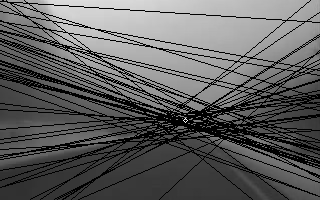
\includegraphics[scale=\imTrackScale]{images/bF_0000_50.png}
	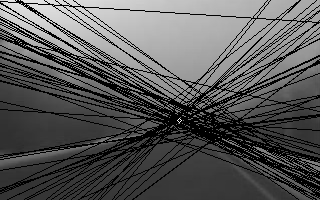
\includegraphics[scale=\imTrackScale]{images/bF_0020_50.png}
	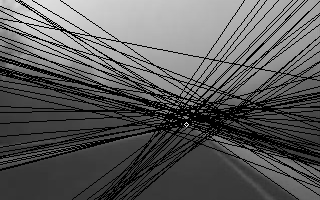
\includegraphics[scale=\imTrackScale]{images/bF_0040_50.png}
	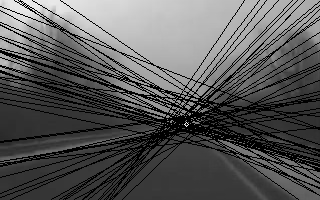
\includegraphics[scale=\imTrackScale]{images/bF_0060_50.png}
\end{minipage}
\begin{minipage}[c]{0.5\linewidth}
	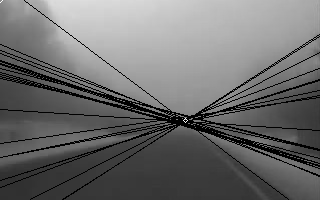
\includegraphics[scale=\imTrackScale]{images/aF_0000_50.png}
	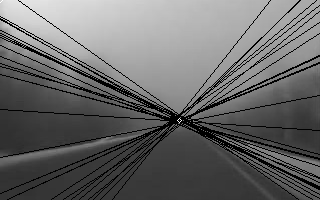
\includegraphics[scale=\imTrackScale]{images/aF_0020_50.png}
	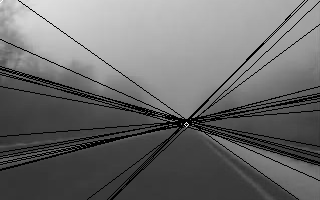
\includegraphics[scale=\imTrackScale]{images/aF_0040_50.png}
	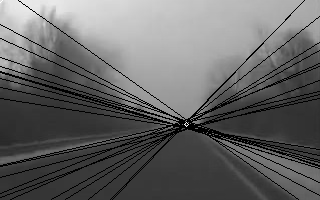
\includegraphics[scale=\imTrackScale]{images/aF_0060_50.png}
\end{minipage}
\caption[short]{A sinistra: linee di fuga per 50 frames a partire dalle immagini 0, 20, 40 e 60. A destra: stesse features dopo il filtro sul vanishing point.}
\label{fig:vp50}
\end{figure}



\section{Stima di $\lambda$ mediante fitting}

\newcommand{\imFeatScale}{0.31}
\newcommand{\imFeatAngle}{0}
\begin{figure}
\begin{minipage}[t]{0.3\linewidth}
	\centering
	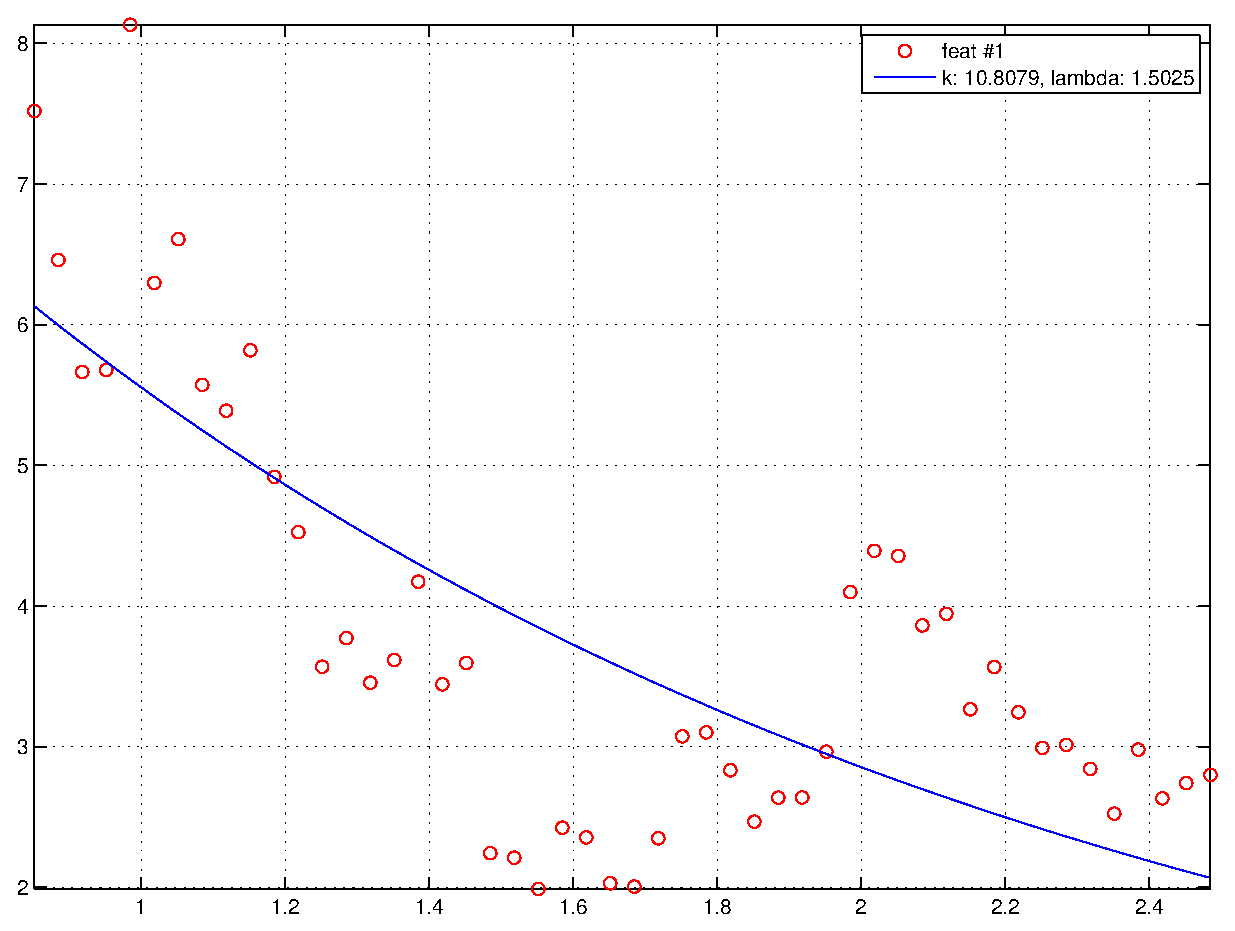
\includegraphics[scale=\imFeatScale, angle=90]{images/feat1}
	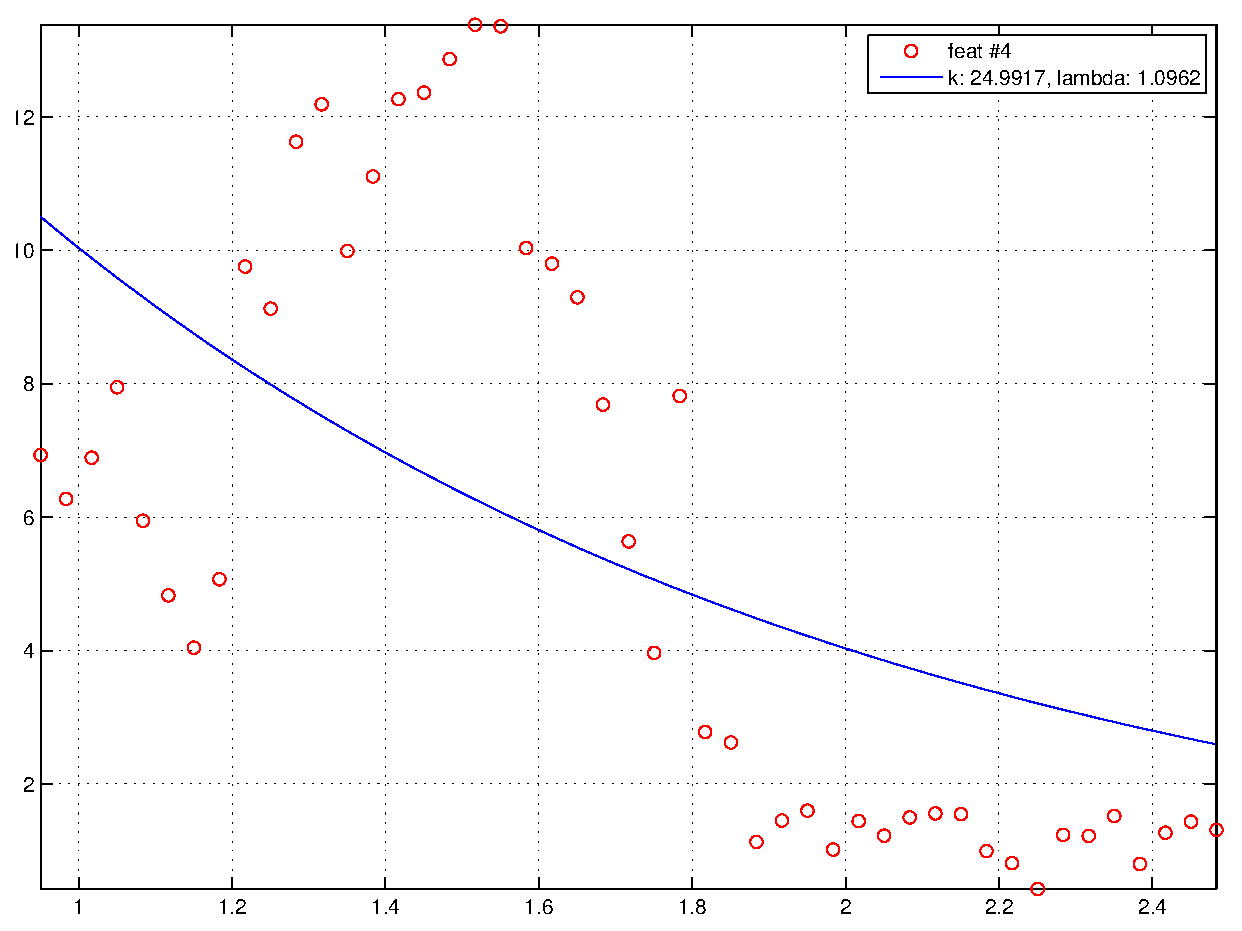
\includegraphics[scale=\imFeatScale, angle=90]{images/feat4}
	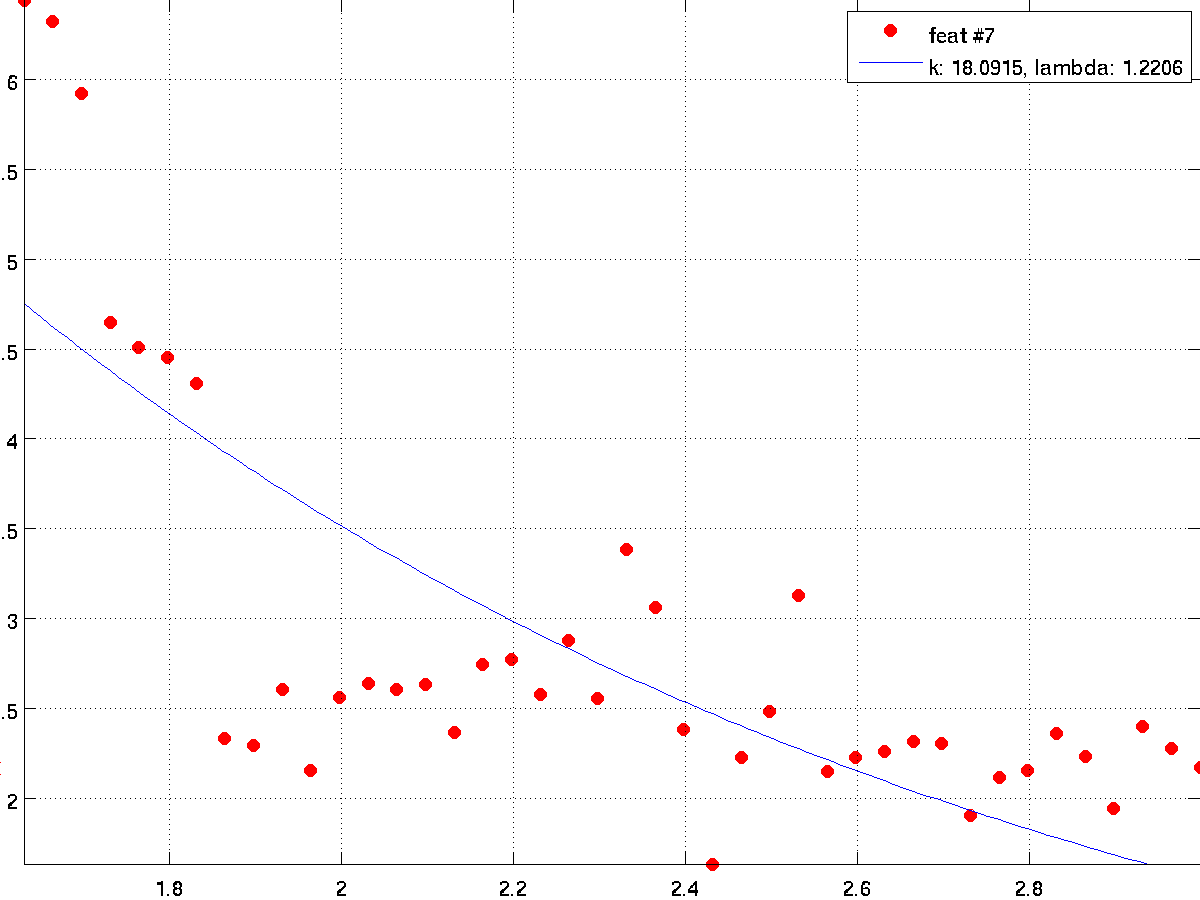
\includegraphics[scale=\imFeatScale, angle=90]{images/feat7}
\end{minipage}
\begin{minipage}[t]{0.3\linewidth}
	\centering
	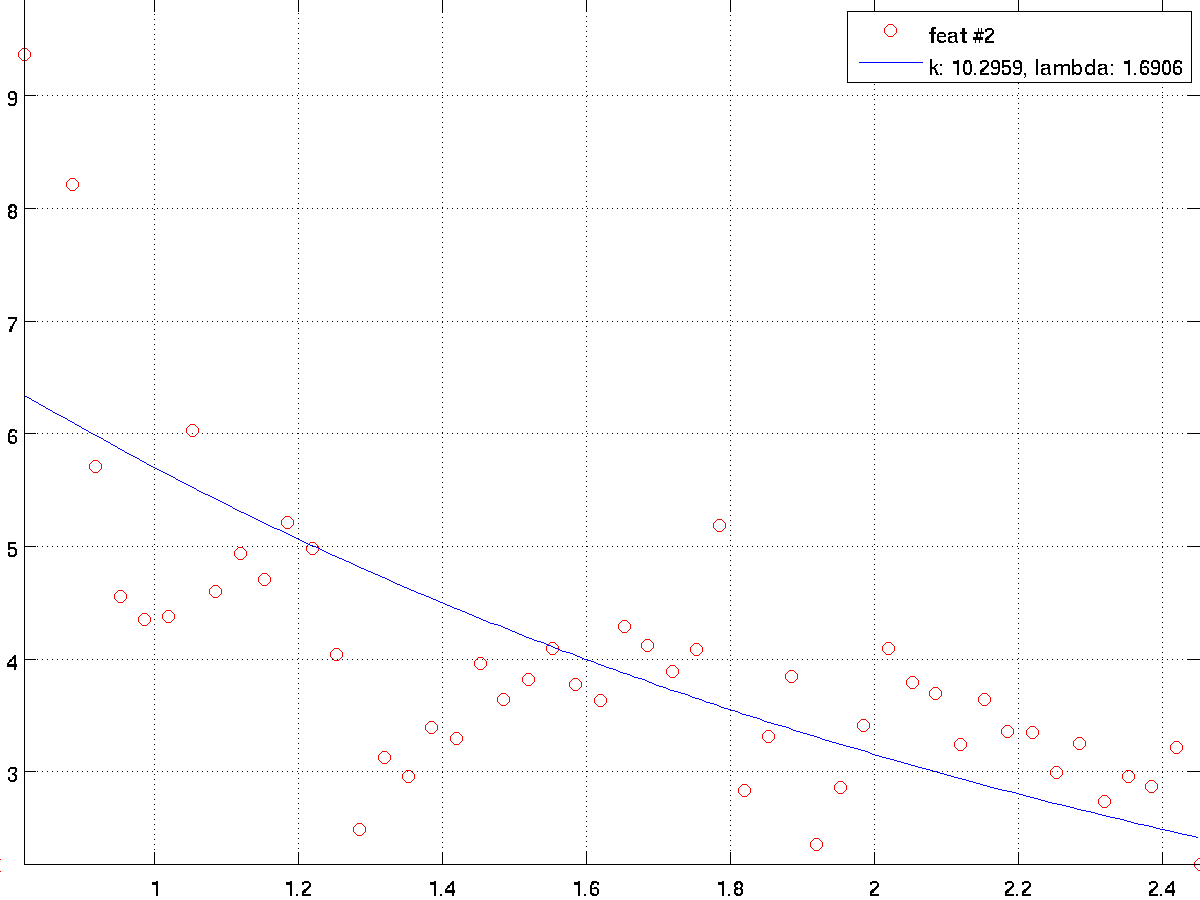
\includegraphics[scale=\imFeatScale, angle=90]{images/feat2}
	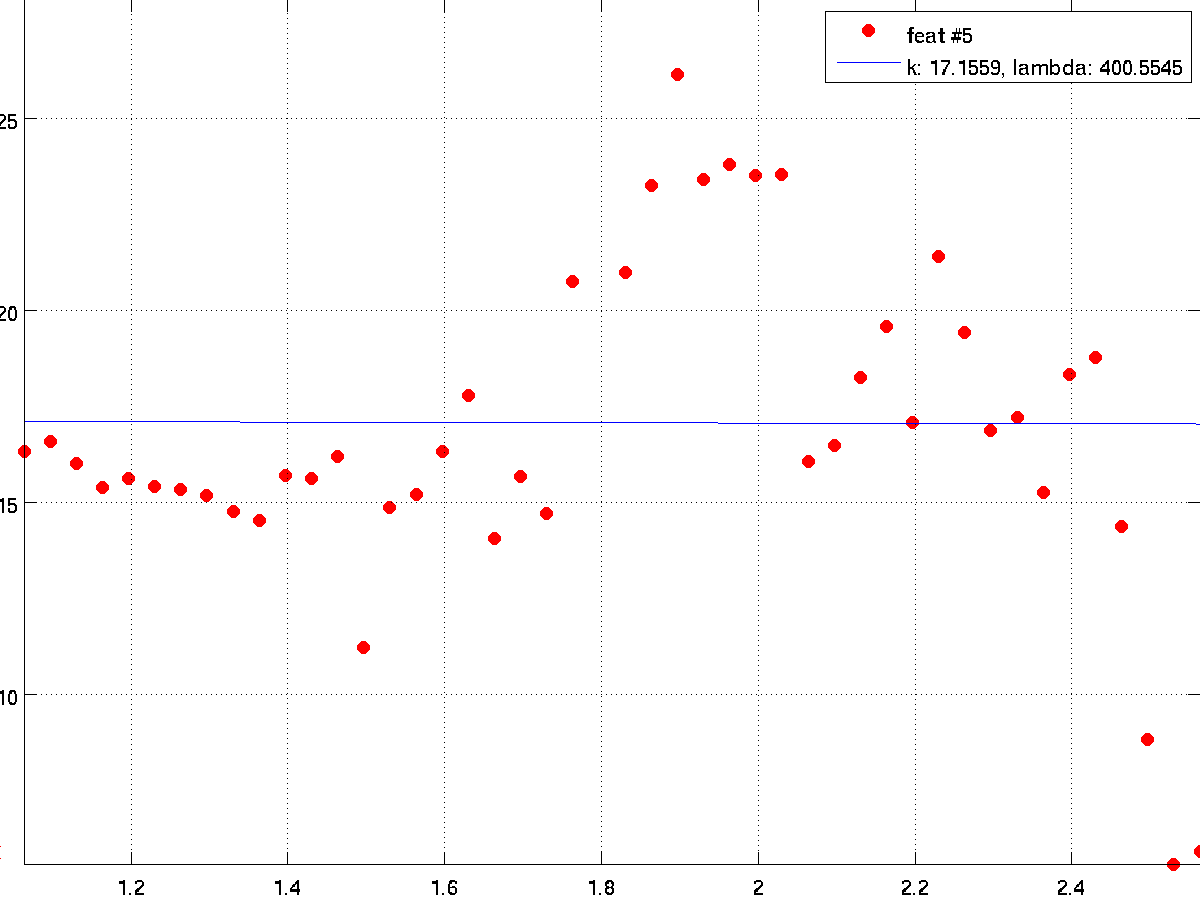
\includegraphics[scale=\imFeatScale, angle=90]{images/feat5}
	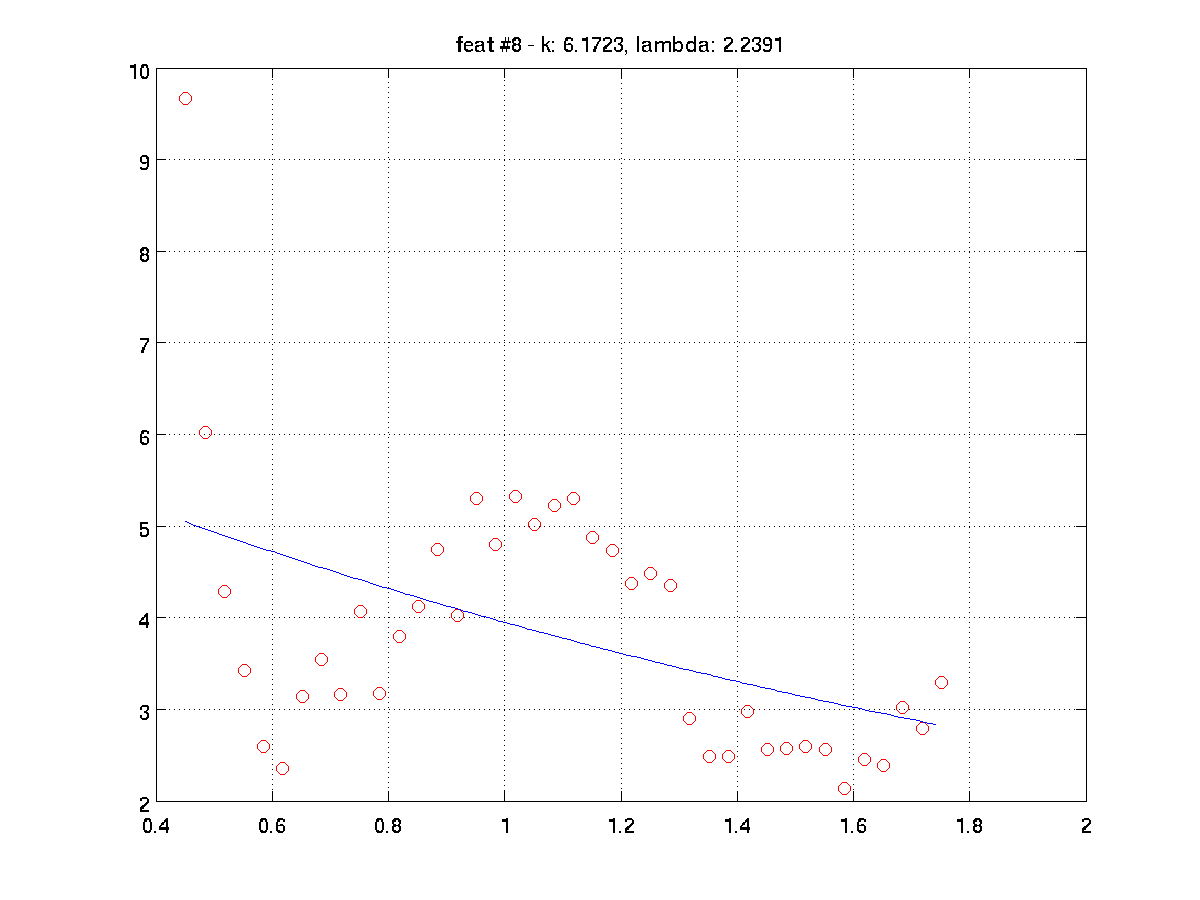
\includegraphics[scale=\imFeatScale, angle=90]{images/feat8}
\end{minipage}
\begin{minipage}[t]{0.3\linewidth}
	\centering
	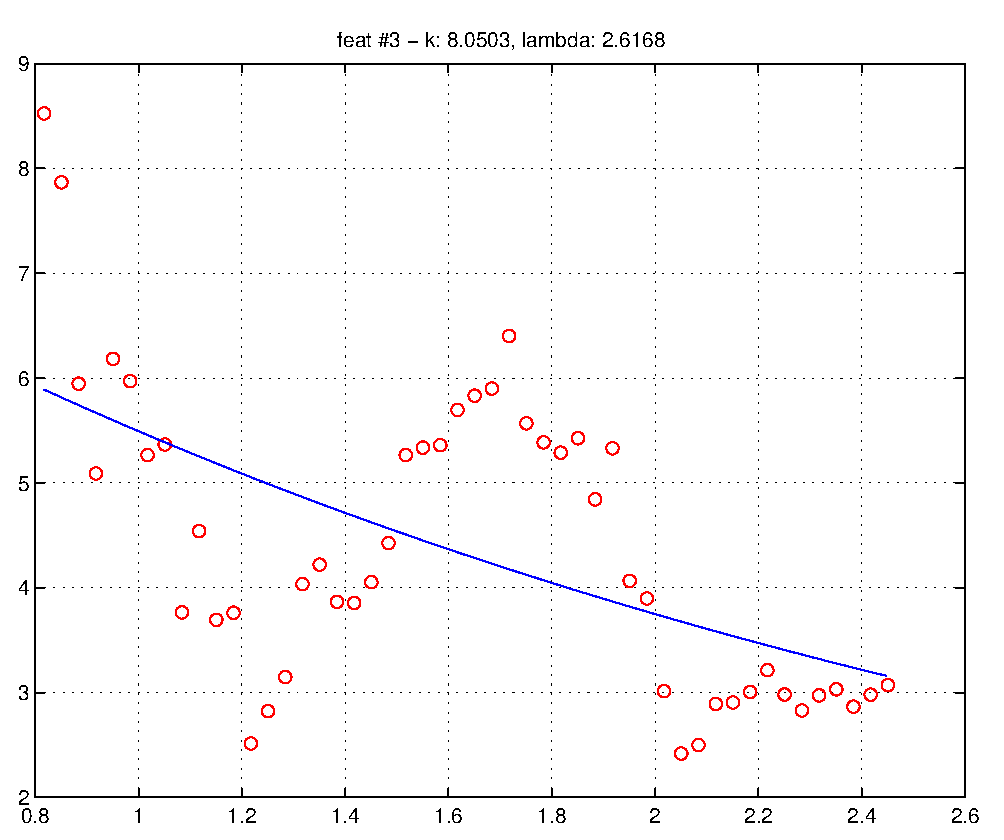
\includegraphics[scale=\imFeatScale, angle=90]{images/feat3}
	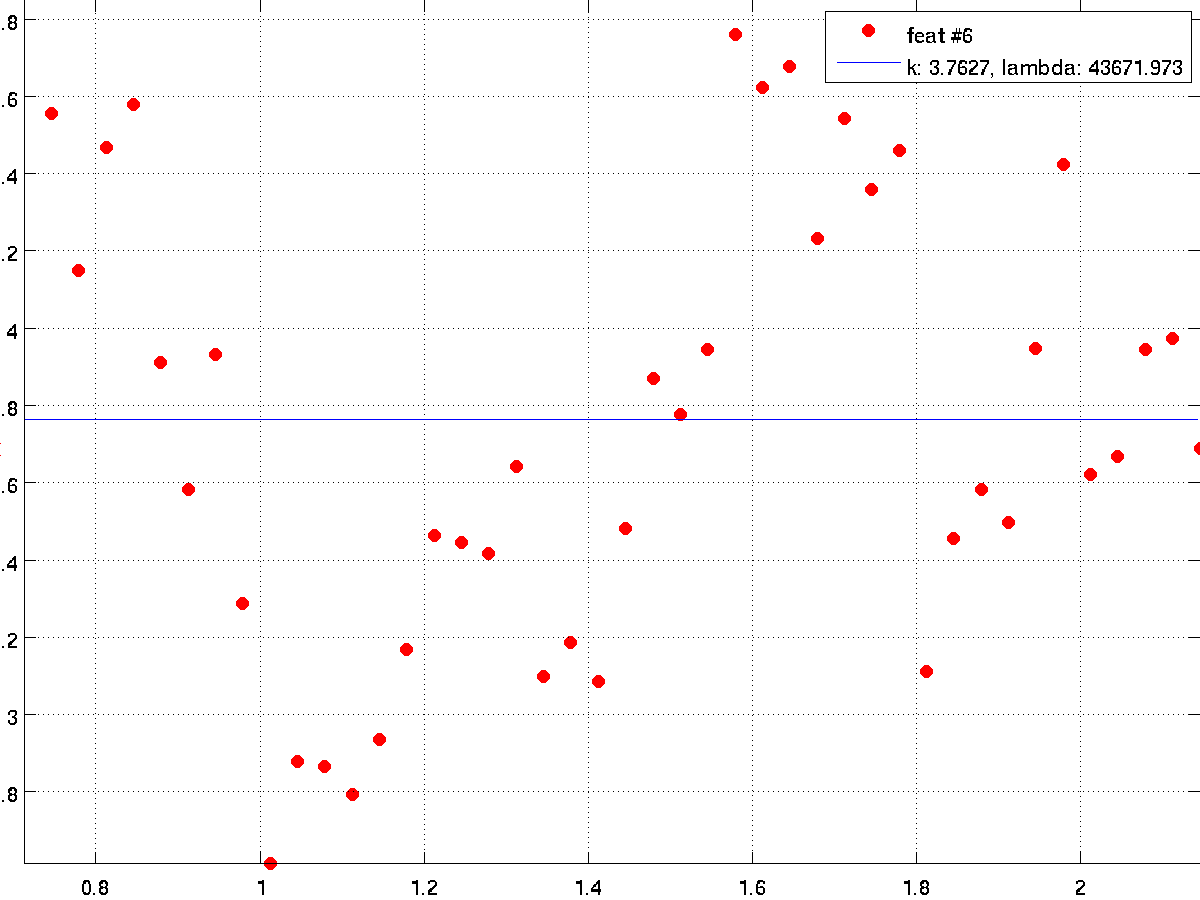
\includegraphics[scale=\imFeatScale, angle=90]{images/feat6}
	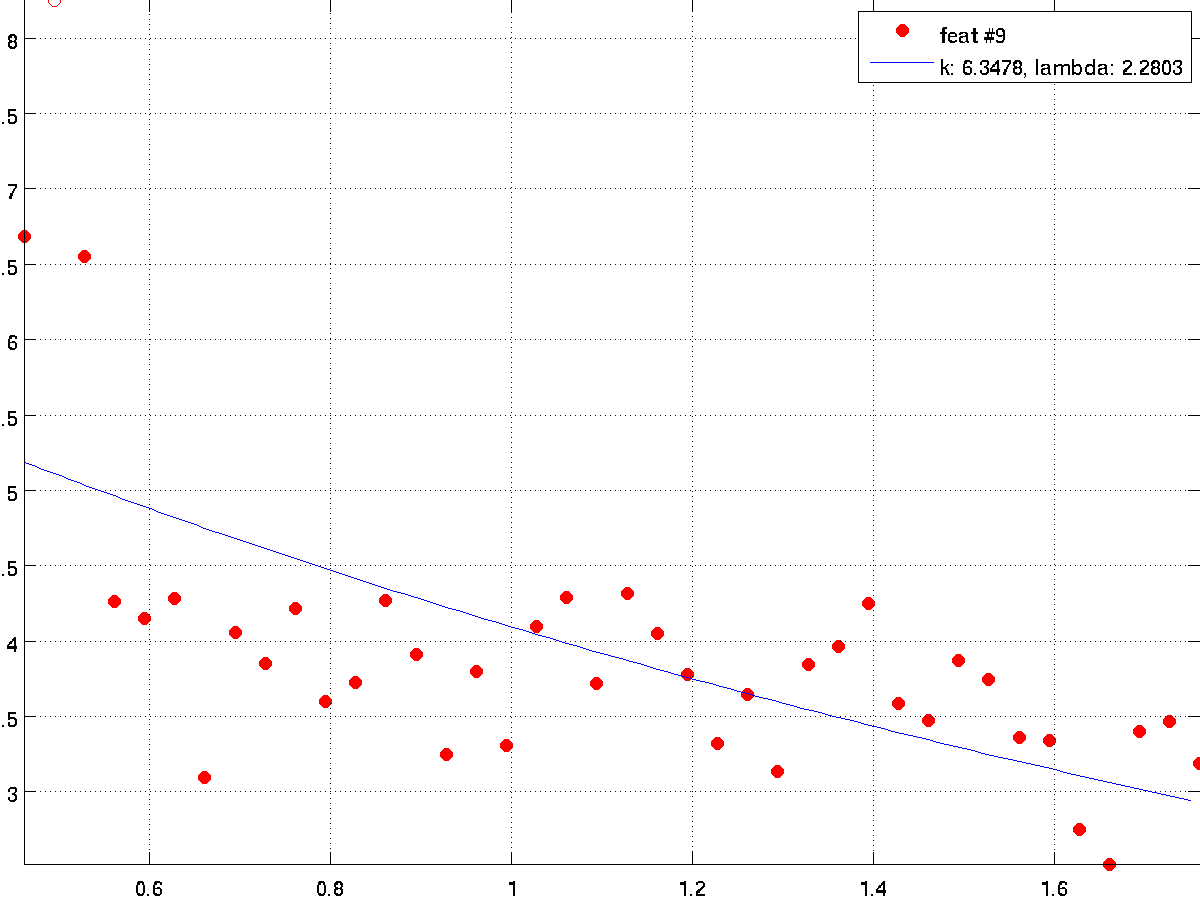
\includegraphics[scale=\imFeatScale, angle=90]{images/feat9}
\end{minipage}
\caption[short]{Features. In ascissa il tempo all'impatto.}
\label{fig:feats}
\end{figure}

\begin{figure}
\begin{minipage}[t]{0.5\linewidth}
	\centering
	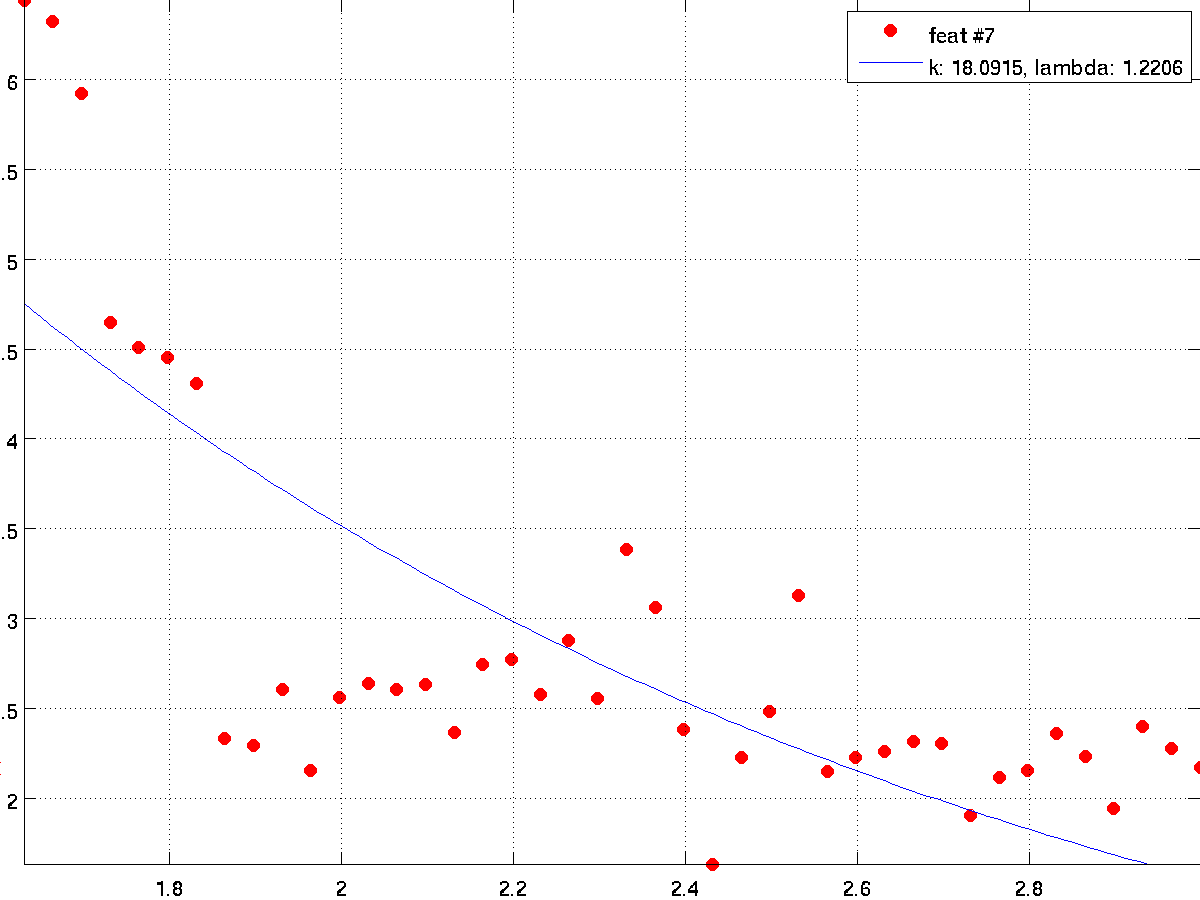
\includegraphics[scale=\imFeatScale, angle=\imFeatAngle]{images/feat7}
	feat7 - $k: , \lambda:  $\\
	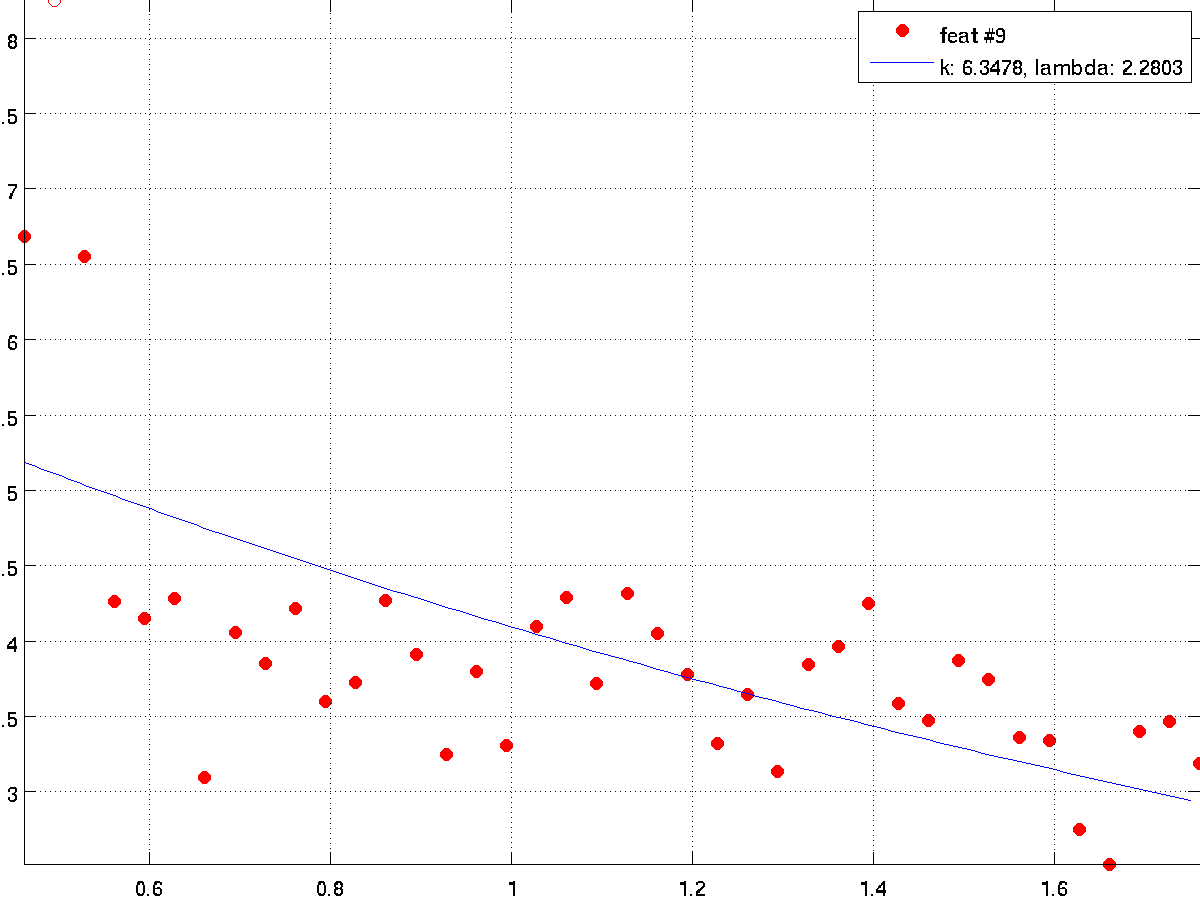
\includegraphics[scale=\imFeatScale, angle=\imFeatAngle]{images/feat9}
	feat9 - $k: , \lambda:  $\\
	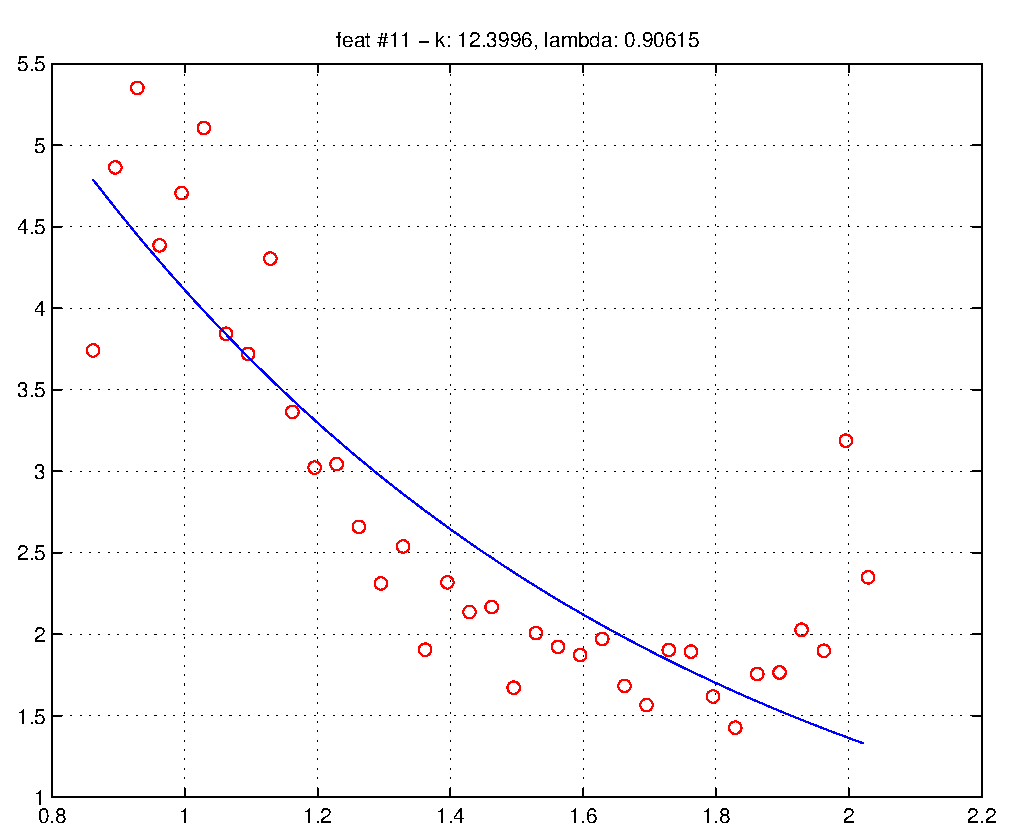
\includegraphics[scale=\imFeatScale, angle=\imFeatAngle]{images/feat11}
	feat11 - $k: , \lambda:  $\\
\end{minipage}
\begin{minipage}[t]{0.5\linewidth}
	\centering
	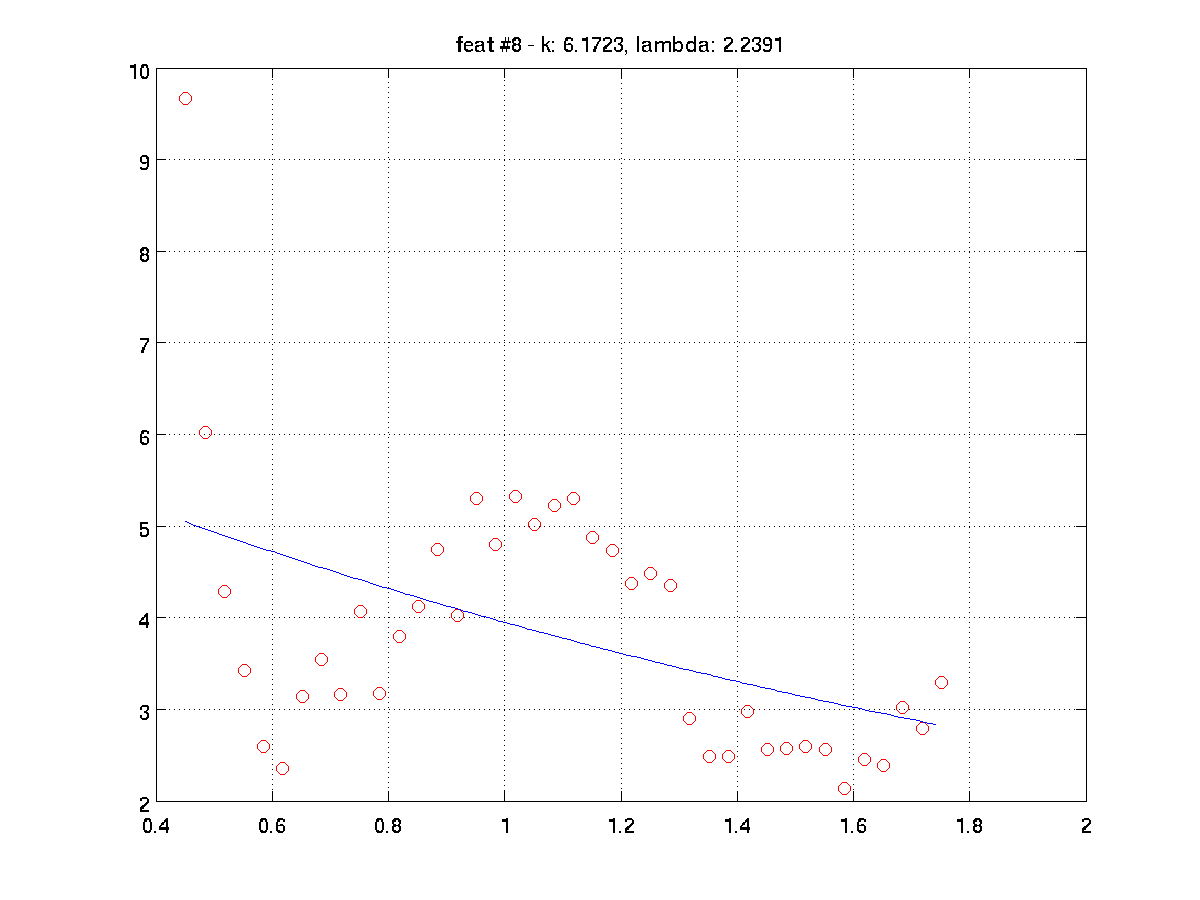
\includegraphics[scale=\imFeatScale, angle=\imFeatAngle]{images/feat8}
	feat8 - $k: , \lambda:  $\\
	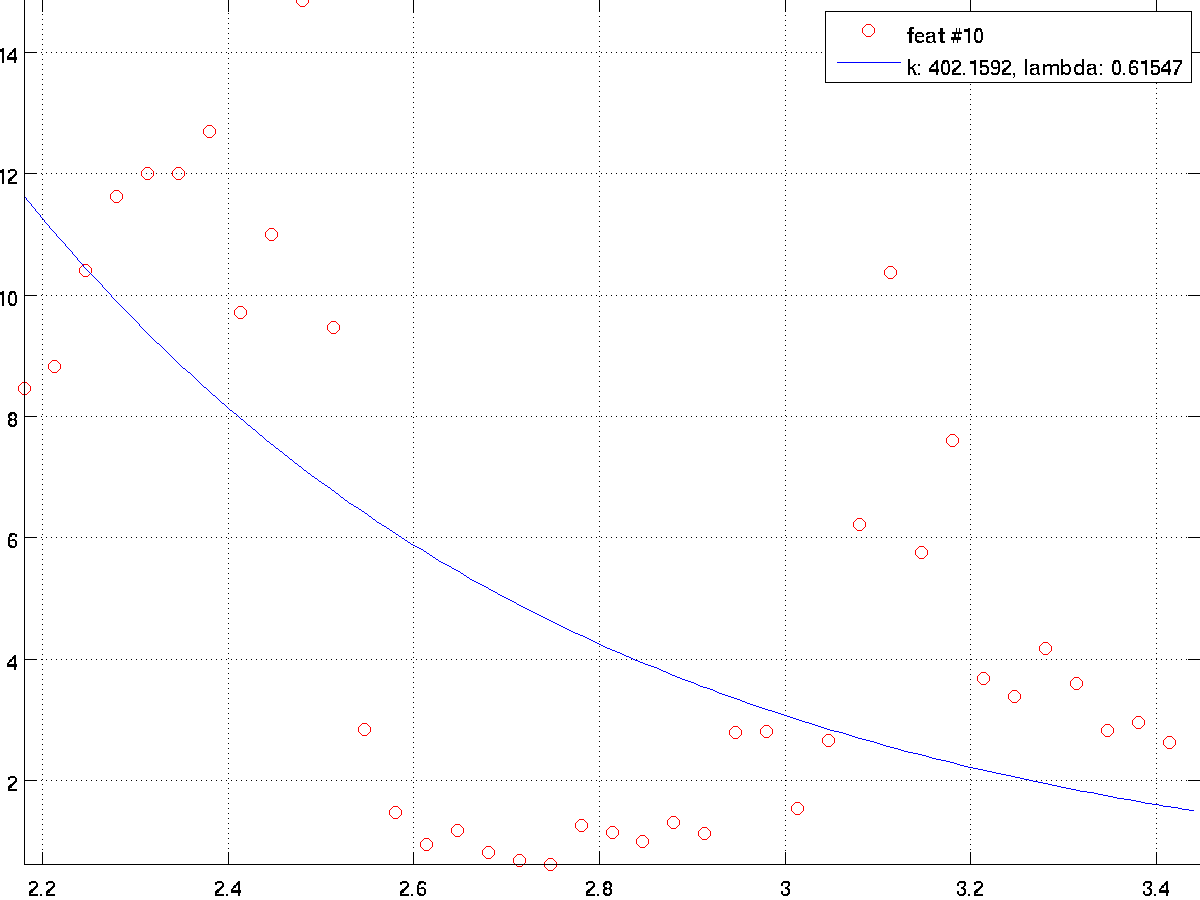
\includegraphics[scale=\imFeatScale, angle=\imFeatAngle]{images/feat10}
	feat10 - $k: , \lambda:  $\\
	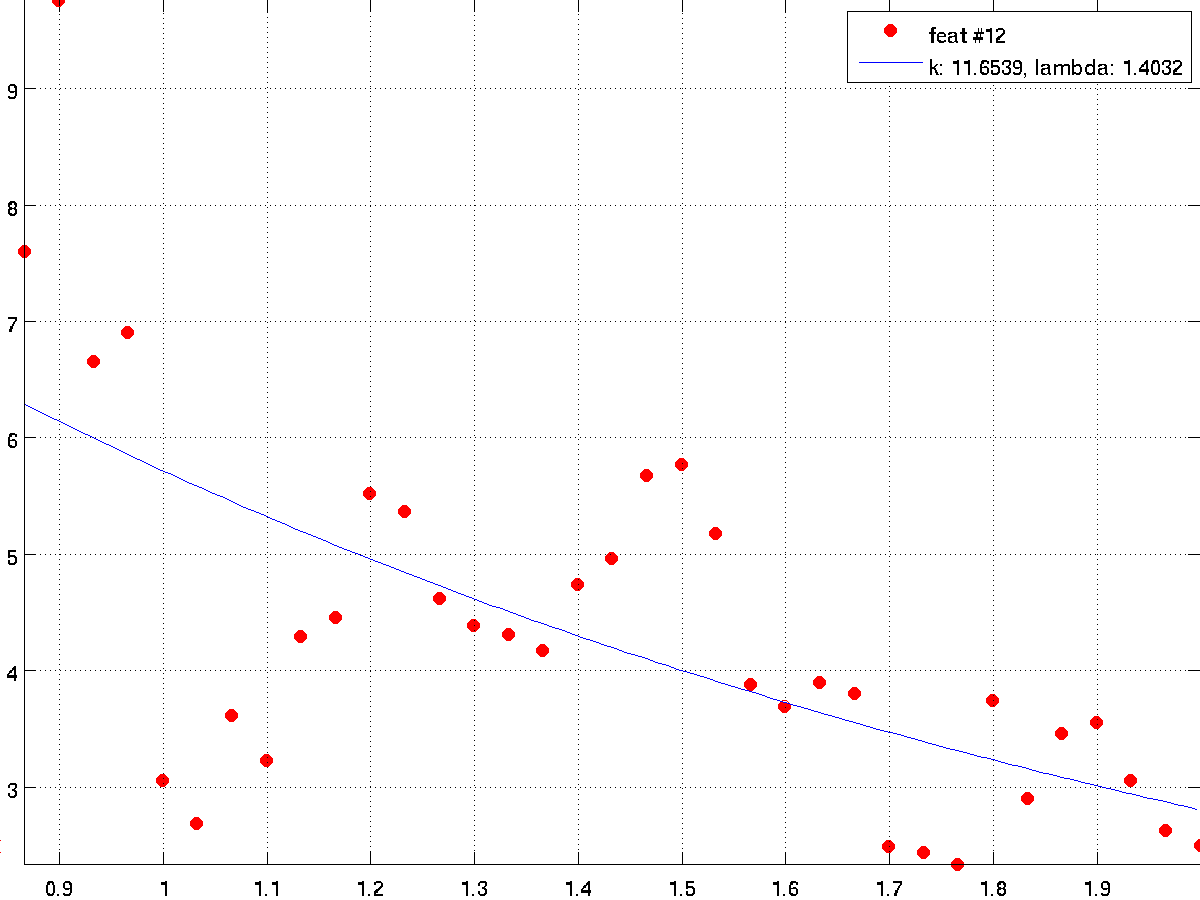
\includegraphics[scale=\imFeatScale, angle=\imFeatAngle]{images/feat12}
	feat12 - $k: , \lambda:  $\\
\end{minipage}
\caption[short]{Features. In ascissa il tempo all'impatto.}
\label{fig:feats2}
\end{figure}

\begin{figure}
\begin{minipage}[t]{0.3\linewidth}
	\centering
	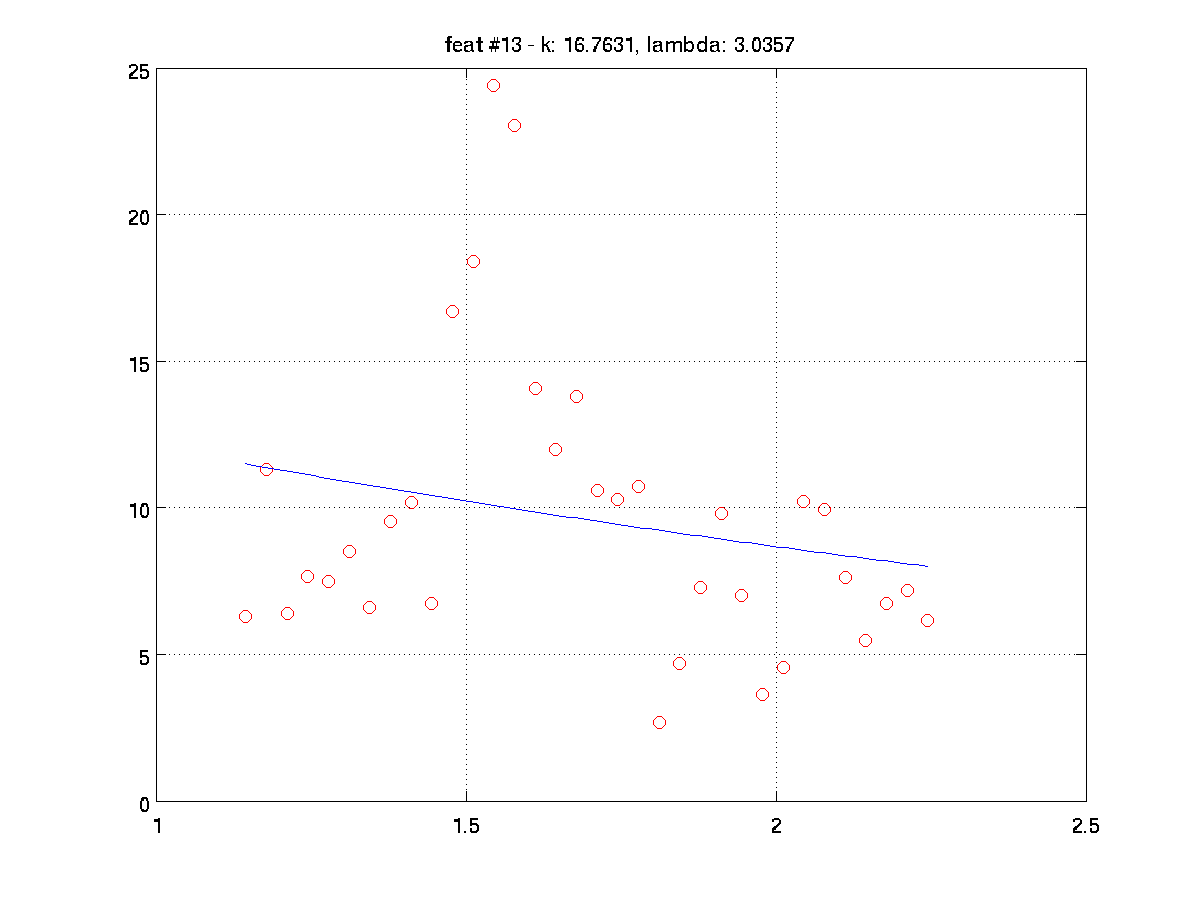
\includegraphics[scale=\imFeatScale]{images/feat13}
	feat7 - $k: , \lambda:  $\\
	\includegraphics[scale=\imFeatScale]{images/feat15}
	feat9 - $k: , \lambda:  $\\
	\includegraphics[scale=\imFeatScale]{images/feat17}
	feat11 - $k: , \lambda:  $\\
\end{minipage}
\begin{minipage}[t]{0.3\linewidth}
	\centering
	\includegraphics[scale=\imFeatScale]{images/feat14}
	feat8 - $k: , \lambda:  $\\
	\includegraphics[scale=\imFeatScale]{images/feat16}
	feat10 - $k: , \lambda:  $\\
	\includegraphics[scale=\imFeatScale]{images/feat18}
	feat12 - $k: , \lambda:  $\\
\end{minipage}
\begin{minipage}[t]{0.3\linewidth}
	\centering
	\includegraphics[scale=\imFeatScale]{images/feat14}
	feat8 - $k: , \lambda:  $\\
	\includegraphics[scale=\imFeatScale]{images/feat16}
	feat10 - $k: , \lambda:  $\\
	\includegraphics[scale=\imFeatScale]{images/feat18}
	feat12 - $k: , \lambda:  $\\
\end{minipage}
\caption[short]{Features. In ascissa il tempo all'impatto.}
\label{fig:feats3}
\end{figure}

\begin{figure}
\begin{minipage}[t]{0.5\linewidth}
	\centering
	\includegraphics[scale=\imFeatScale]{images/feat19}
	feat7 - $k: , \lambda:  $\\
\end{minipage}
\begin{minipage}[t]{0.5\linewidth}
	\centering
	\includegraphics[scale=\imFeatScale]{images/feat20}
	feat8 - $k: , \lambda:  $\\
\end{minipage}
\caption[short]{Features. In ascissa il tempo all'impatto.}
\label{fig:feats4}
\end{figure}




\chapter{Conclusioni e sviluppi futuri}

\noindent I risultati dei test hanno evidenziato come il problema sia fortemente influenzato dal numero di outliers derivati sia un errato tracking delle features, sia da una non perfetta variazione del contrasto sulle features stesse. Il maggior sforzo computazionale \`e infatti da attribuire alla complessit\`a degli algoritmi utilizzati per escludere gli outliers in tutte le fasi dell'elaborazione in modo da avere valori attendibili in ogni condizione.\\

\noindent Sono stati analizzati diversi approcci ed algoritmi per la risoluzione del problema, e si \`e preferito, in ultimo, sacrificare il tempo di elaborazione in favore di una migliore affidabilit\`a dei risultati: gli algoritmi utilizzati sono in grado di individuare autonomamente le features migliori e scartare quelle meno buone, ottenendo dei buoni risultati come esposto nei capitoli precedenti.\\

\noindent Possibili sviluppi futuri possono riguardare la reimplementazione in C\verb|++| del codice Matlab ed un'ottimizzazione degli algoritmi mirata a migliorarne le performance, eventualmente fino al punto di rendere possibile l'analisi direttamente su uno streaming video in realtime, senza le rielaborazioni successive del codice attualmente in uso.





\chapter{Documentazione}


Viene qui presentata una panoramica delle funzioni realizzate. Per informazioni pi\`u dettagliate circa il loro utilizzo consultare l'\verb|help| delle funzioni.

\section[C++]{C\verb_++_}

\paragraph*{\verb_findFeatures:_} \`e la funzione principale dell'algoritmo, si occupa di chiamare le sottoprocedure dell'algoritmo

\paragraph*{\verb_iaasFindCorners:_} estrae dall'immagine i corner con autovalori pi\`u alti

\paragraph*{\verb_iaasTrackCorners:_} cerca di rintracciare i corner della prima immagine (gi\`a calcolati) nella seconda utilizzando l'algoritmo di \emph{Lucas-Kanade}

\paragraph*{\verb_verifyNewFeatureIsOk:_} verifica che un nuovo corner estratto sia coerente con quelli in precedenza rilevati

\paragraph*{\verb_getAroundContrast:_} calcola il contrasto nell'intorno di una feature usando RMS: $$ c\left(I_{M\times N}\right) = \sqrt{\frac{1}{MN}\sum_{i=1}^N\sum_{j=1}^M(i_{ij}-\bar{I})^2} $$

\paragraph*{\verb_verifyValidFeature:_} verifica che una sequenza di corner estratti sia coerente con il movimento e la cross ratio attesa

\paragraph*{\verb_printFeatures:_} scrive sul file la lista di features valide come:
\begin{verbatim}
	     primoFrame numeroFrame [xCoord yCoord contrasto tti]+
\end{verbatim}


\section{Matlab}

\paragraph*{\verb_iaas:_} funzione principale, parsa le feature generate dal codice C\verb|++| e chiede all'utente di selezionare l'algoritmo per il calcolo del $\lambda$ globale.

\paragraph*{\verb_parseFeatures:_} effettua il parsing del file di output generato da \verb|printFeatures| e restituisce una lista di struct contenente le informazioni di ogni feature: \verb|start| \`e il numero della prima immagine in cui appare la feature, \verb|num| il numero di frame nei quali viene inseguita, \verb|x|, \verb|y|, \verb|contr| e \verb|tti| sono array rappresentanti le coordinate, il contrasto e il tempo all'impatto della feature all'interno nell'i-esimo frame in cui vengono individuate. Nelle seguenti funzioni, quando si far\`a riferimento a liste di features si intender\`a cos\`i strutturate.

\paragraph*{\verb_fitLamContr:_} calcola i parametri della curva best fit sui dati di ciascuna delle features fornite in ingresso, aggiungendo il campo \verb|bestData| degli indici del $50\%$ dei corner con valori di contrasto con errore minimo rispetto alla stima. Viene poi aggiunto l'attributo \verb|pars| contenente i parametri del refitting usando il set \verb|bestData|. Vengono inoltre aggiunti diversi attributi per stimare la bont\`a del set di dati che compongono la singola feature (per una lista esaustiva si rimanda all'help della funzione), fra i quali in particolare ricordiamo \verb|intErr|, che calcola l'area fra le curve dei due successivi fit.

\paragraph*{\verb_estimateLamFit:_} seleziona il quartile delle migliori features usando uno degli attributi calcolati da \verb|fitLamContr| (nel nostro caso abbiamo preferito usare l'errore integrale) e usa la mediana dei $\lambda_f$ stimati per calcolare il parametro globale.

\paragraph*{\verb_fitNormContr:_} calcola il $\lambda$ globale mediante RANSAC dopo aver riscalato i livelli di contrasto di ogni feature in base al valore $k_f$ della curva best fit.

\paragraph*{\verb_normContrast:_} normalizza il contrasto di ogni set di features utilizzando diverse possibili tecniche (per una lista completa si rimanda all'help della funzione). Riportiamo l'opzione \verb|fit|, dal momento che \`e quella pi\`u efficace (e di fatto utilizzata all'interno del progetto), che riscala i contrasti delle singole features in base al $k_f$ della curva che meglio approssima il set di dati.

\paragraph*{\verb_myRansac:_} implementazione di RANSAC per calcolare il parametro $\lambda$ della funzione del contrasto dati in ingresso una lista di features.

\paragraph*{\verb_inspectFeatures:_} stampa a video le sequenze di features per un'ispezione visiva, visualizzandone i relativi valori di contrasto.

\paragraph*{\verb_inspectContrasts:_} data una serie di features ne stampa a video i livelli di contrasto ordinati sul tempo d'impatto.

\paragraph*{\verb_michelsonContrast:_} date le coordinate di una feature e la relative immagine restituisce il livello di contrasto nell'intorno come $$c\left(I\right) = \frac{\max(I)-\min(I)}{\max(I)+\min(I)}$$

\paragraph*{\verb_rsmContrast:_} date le coordinate di una feature e la relativa immagine calcola il livello di contrasto nell'intorno come $$ c\left(I_{M\times N}\right) = \sqrt{\frac{1}{MN}\sum_{i=1}^N\sum_{j=1}^M(i_{ij}-\bar{I})^2} $$

\paragraph*{\verb_weberContrast:_} date le coordinate di una feature e la relative immagine calcola il livello di contrasto come $$c\left(i_{i,j}\right)= \frac{i_{i,j}-I_b}{I_b}$$ dove $I_b$ \`e il livello della nebbia.



\chapter{Installazione}
\noindent Il programma \`e stato sviluppato per mezzo di C\verb|++| e Matlab. Per la parte in C\verb|++| \`e necessario essere provvisti delle librerie di OpenCV.\\
L'ultima versione del codice \`e liberamente scaricabile mediante SVN dalla repository messa a disposizione su Google Code all'indirizzo \url{http://code.google.com/p/iaasfog}.
\section{OpenCV}

OpenCV (Open Source Computer Vision) \`e una libreria di funzioni per la computer vision, inizialmente sviluppata da Intel e ora distribuita sotto licenza open source. \`E possibile scaricare l'ultima versione all'indirizzo \url{http://sourceforge.net/projects/opencvlibrary/} \footnote{guida d'installazione ufficiale all'indirizzo \url{http://opencv.willowgarage.com/wiki/InstallGuide}}.

\subsection{Windows}

Per compilare la libreria \`e necessario installare gli header offerti da MinGW (\url{http://http://www.mingw.org/}) e CMake (\url{http://www.cmake.org/cmake/resources/software.html}).\\
\noindent Una volta assicuratisi che il path dei binari di MinGW \`e fra le variabili di ambiente configurare OpenCV mediante l'interfaccia di CMake.

\subsection{Linux / MacOSX}

\noindent Per l'installazione \`e necessario disporre di \verb|cmake|, inoltre devono essere soddisfatte le seguenti dipendenze:
\begin{itemize}
\item \verb|ffmpeg|
\item \verb|libxine-ffmpeg|
\item \verb|libavcodec-dev|
\item \verb|pgk-config|
\item \verb|libgtk2.0-dev|
\end{itemize}

\noindent reperibili mediante \verb|apt-get| o package manager.\\

\noindent Una volta scaricata e scompattata l'ultima versione di OpenCV (2.2.0 alla stesura del presente documento), creare una cartella dove verranno salvate le librerie configurate mediante \verb|cmake| e aprirla con una finestra di terminale. Nel nostro esempio la creeremo nella stessa cartella scompattata

\begin{verbatim}
	$ cd OpenCV2.2.0/
	$ mkdir release; cd release
\end{verbatim}

\noindent Lanciare quindi il comando

\begin{verbatim}
	$ cmake -D CMAKE_BUILD_TYPE=RELEASE -D CMAKE_INSTALL_PREFIX=/usr/local
	-D BUILD_PYTHON_SUPPORT=ON -D BUILD_EXAMPLES=ON ..
\end{verbatim}

\noindent per configurare la libreria. Il valore della flag \verb|CMAKE_INSTALL_PREFIX| sar\`a l'indirizzo in cui si vorr\`a poi installare OpenCV. Se i sorgenti non dovessero trovarsi nella directory superiore, sostituire i due punti con il path corretto.\\

\noindent A questo punto non rimane che compilare ed installare le librerie mediante i comandi

\begin{verbatim}
	$ make
	$ make install
\end{verbatim}

\noindent ed esportare il path nelle variabili di ambiente con il comando

\begin{verbatim}
	$ export LD_LIBRARY_PATH=/usr/local/lib/:$LD_LIBRARY_PATH
	$ sudo ldconfig
\end{verbatim}

\noindent Se invece si preferisce non installare le librerie, esportare direttamente il path 

\begin{verbatim}
	$ export LD_LIBRARY_PATH=<opencv_dir>:$LD_LIBRARY_PATH
	$ sudo ldconfig
\end{verbatim}

\noindent dove \verb|<opencv_dir>| \`e la cartella dove abbiamo compilato le librerie, nel nostro caso \verb|~/OpenCV-2.2.0/release|.

\section{Installazione ed esecuzione del programma}

\noindent Dopo aver scaricato il progratto da \url{http://code.google.com/p/iaasfog}, importare i sorgenti nella cartella C\verb|++| in Eclipse, importare gli header delle funzioni di OpenCV mediante Project $\rightarrow$ Properties  $\rightarrow$ C\slash C\verb|++| Editor $\rightarrow$ Settings $\rightarrow$ GCC C\verb|++| Compiler $\rightarrow$ Directories aggiungendo il percorso \verb|/usr/local/include/| e sotto GCC C\slash C\verb|++| Linker $\rightarrow$ Libraries le librerie \verb|opencv_core|, \verb|opencv_video|, \verb|opencv_highgui| e \verb|opencv_imgproc| in \verb|/usr/local/lib| (o qualunque path sia stato utilizzato per l'installazione).\\
Compilare.\\

\noindent In Matlab aggiungere il path degli m-file ed assicurarsi che il percorso specificato dalla varibile \verb|exec_path| in \verb|iaas.m| corrisponda alla cartella dell'eseguibile del codice C\verb|++|.\\
Per eseguire il programma lanciare nella console di Matlab il comando \verb|iaas [#]|, dove \verb|#|, opzionale, non far\`a visualizzare nessuna finestra se assente o uguale a \verb|0|, se uguale a \verb|1| visualizzer\`a una serie di grafici che mostrano le curve approssimanti, mentre se uguale a \verb|2| mostrer\`a un numero maggiore di grafici (modalit\`a pensata principalmente per il debugging, l'eccessiva quantitat\'a di grafici rischia di risultare tediosa per l'utente).

%\printbibliography

\end{document}
